\documentclass[11pt]{article}

\usepackage[a4paper, margin=1in]{geometry}
\usepackage[utf8]{inputenc}
\usepackage[T1]{fontenc}
\usepackage{microtype}
\usepackage{amsmath, amssymb, amsthm}
\usepackage{booktabs}
\usepackage{multirow}
\usepackage{graphicx}
\usepackage{hyperref}
\usepackage{natbib}
\usepackage{authblk}
\usepackage{float}
\usepackage{xcolor}

\hypersetup{
  colorlinks=true,
  linkcolor=blue!50!black,
  citecolor=blue!50!black,
  urlcolor=blue!50!black,
}

\title{\bf HAR-RV Holds Up: A Multi-Horizon Walk-Forward Benchmark of \\
Classical, Tree-Based, and Deep Volatility Forecasts on NIFTY-50}

\author[1]{Manav Mishra\thanks{\texttt{manavmishra260205@gmail.com}}}
\affil[1]{Vellore Institute of Technology, Vellore, India}

\date{\today}

\newtheorem{proposition}{Proposition}

\begin{document}

\maketitle

\begin{abstract}
The HAR-RV model of \citet{corsi2009} is widely reported as
difficult to beat in volatility forecasting. We provide a controlled
walk-forward comparison of five models---GARCH(1,1), HAR-RV, XGBoost,
LSTM, and a Transformer encoder---on NIFTY-50 daily realized
volatility from September 2007 through June 2026 (4{,}585 trading
days; 3{,}500+ out-of-sample forecasts per model), evaluated at
forecast horizons of 1, 5, and 22 trading days. Our primary metric is
the QLIKE loss \citep{patton2011}, and we use Diebold--Mariano tests
\citep{dieboldmariano1995} computed on QLIKE-per-observation losses
to maintain consistency between evaluation and significance testing.
Across all three horizons and four challenger models, \emph{no model
achieves a statistically significant improvement over HAR-RV under
QLIKE-based DM tests}. Numerical QLIKE values do favor sequence
models at the one-day horizon (LSTM 0.600 vs HAR 0.625) and
GARCH-style mean-reverting forecasts at the 22-day horizon (GARCH
0.760 vs HAR 0.969), but these differences fall within the noise
band of DM testing on this single-index sample. At the 5-day
horizon, XGBoost is the only model with a statistically significant
result---and it is significantly \emph{worse} than HAR. Our
numerical direction agrees with the recent ML-beats-HAR finding of
\citet{christensen2023machine} on the cross-section of DJIA
constituents, but our single-index sample lacks the statistical
power to confirm the result at conventional significance levels
under QLIKE-based DM. The findings highlight the importance of
using a single loss function consistently for both evaluation and
significance testing, and they suggest that single-asset replications
of cross-sectional ML-vs-HAR studies should be interpreted with the
sample-power caveat in mind.
\end{abstract}

\section{Introduction}
\label{sec:intro}

Volatility forecasting is a cornerstone problem in quantitative
finance. Forecasts of conditional return variance are required as
inputs to option-pricing models \citep{black1973pricing},
value-at-risk and expected-shortfall computations, and a wide range
of allocation and hedging procedures \citep{andersen2006volatility}.
The literature spans nearly four decades, anchored by
\citet{engle1982arch} and \citet{bollerslev1986garch}, and refined
through asymmetric and long-memory variants such as EGARCH
\citep{nelson1991egarch} and Realized GARCH
\citep{hansen2012realized}.

Since the introduction of \emph{realized variance} estimators
\citep{andersen2003modeling}, the dominant benchmark in volatility
forecasting has been the Heterogeneous Autoregressive model of
realized variance (HAR-RV) of \citet{corsi2009}. HAR-RV is a
parsimonious linear regression on lagged daily, weekly, and monthly
aggregates of realized variance. Its persistent empirical advantage
has motivated a substantial literature attempting to beat it with
richer specifications or machine-learning models
\citep{audrino2020machine, christensen2023machine}.
\citet{christensen2023machine}, in the most comprehensive recent
US-data benchmark, find that machine learning is competitive with
and beats the HAR lineage on the cross-section of Dow Jones
Industrial Average constituents, with gains intensifying at
longer horizons. Earlier studies on individual stocks and
indices report heterogeneous results across markets, sample
windows, and loss functions.

The Indian equity market is underrepresented in this literature.
Volatility forecasting studies on NIFTY-50 have largely focused on
classical GARCH-family specifications; comprehensive deep-learning
benchmarks remain limited. Filling this gap is useful because Indian
markets exhibit distinct features---pronounced overnight effects,
sharp regime shifts around policy and election cycles---that make
them a non-trivial test bed for sequence models.

\paragraph{Contributions.} This paper contributes:

\begin{enumerate}
  \item A controlled walk-forward benchmark of five models on
  18+~years of NIFTY-50 daily data at three forecast horizons
  (1, 5, and 22 trading days), with a uniform initial training
  window and evaluation loss across all models.
  \item Diebold--Mariano significance tests \emph{computed on
  per-observation QLIKE losses}, maintaining consistency between
  our primary loss and our significance metric. We document that
  earlier benchmarks using MSE-on-log-variance for DM testing can
  yield qualitatively different conclusions from QLIKE-based tests
  on the same prediction series.
  \item A reproducible open-source implementation that includes data
  ingestion, all five models, the evaluation harness, robustness
  analyses, and analysis notebooks.\footnote{Source code:
  \url{https://github.com/manavmishra-cloud/nifty-vol-forecast}}
  \item The empirical finding that, on NIFTY-50 daily data,
  \emph{no model statistically beats HAR-RV under QLIKE-based DM
  tests at any horizon}. Numerical QLIKE differences favor sequence
  models at the one-day horizon and GARCH at the 22-day horizon,
  numerically consistent in direction with the US-data finding of
  \citet{christensen2023machine}, but the single-index design
  used here lacks statistical power to confirm a significant
  advantage under QLIKE-based DM testing.
\end{enumerate}

\section{Related Work}
\label{sec:related}

\paragraph{Classical conditional-variance models.} The ARCH family
\citep{engle1982arch, bollerslev1986garch} models the conditional
variance of returns as a function of past squared returns and lagged
variance. Asymmetric variants such as EGARCH \citep{nelson1991egarch}
and GJR-GARCH \citep{glosten1993relation} capture the leverage
effect. These models remain the practical default in many
risk-management contexts.

\paragraph{Realized-variance models.} \citet{andersen2003modeling}
introduce realized variance as the sum of intraday squared returns,
an observable proxy for latent variance. When only daily OHLC data
is available, range-based estimators serve as low-frequency
substitutes: Parkinson \citep{parkinson1980}, Garman-Klass
\citep{garman1980}, Rogers and Satchell \citep{rogers1991}, and Yang
and Zhang \citep{yang2000}. The HAR-RV specification of
\citet{corsi2009} regresses log realized variance on its lagged
daily, weekly, and monthly averages, and \citet{hansen2012realized}
couples returns and realized measures.

\paragraph{Machine learning in volatility forecasting.}
\citet{christensen2023machine} provide an extensive out-of-sample
comparison of tree-based and neural network methods against
HAR-family specifications on the Dow Jones Industrial Average
constituents, finding that machine learning beats the HAR lineage
even when restricted to lagged realized variance as the only
predictor, with gains intensifying at longer horizons. Their
result motivates the present systematic Indian-markets replication
and provides the natural US-data benchmark for our findings.
Earlier studies on individual stocks and indices report
heterogeneous results across markets, sample windows, and loss
functions.

\paragraph{Loss functions and significance testing.}
\citet{patton2011} establishes QLIKE as a robust loss for volatility
forecast evaluation under noisy variance proxies. \citet{patton2009volatility}
emphasizes the importance of consistency between the loss used for
forecast evaluation and the loss used in pairwise significance tests
such as the Diebold--Mariano test. Our paper takes this advice
seriously, with consequences for the conclusions reached.

\paragraph{Deep learning in financial time series.} Beyond
volatility, sequence models have been applied to return prediction
\citep{sirignano2019universal}, option pricing
\citep{horvath2021deep}, and limit order book modeling
\citep{briola2020deep}. \citet{vaswani2017attention} introduce the
Transformer architecture used here.

\section{Data}
\label{sec:data}

We use daily OHLCV for the NIFTY-50 index symbol
\texttt{\textasciicircum NSEI} from Yahoo Finance, covering
2007-09-18 through 2026-06-01 (4{,}585 trading days, 4{,}584 with
computable Yang-Zhang realized variance). NIFTY-50 is the
broad-based Indian large-cap equity index maintained by the National
Stock Exchange of India.

\paragraph{Realized variance estimator.} As we have only daily
OHLCV, we use the range-based Yang-Zhang estimator
\citep{yang2000}:
\begin{align}
\sigma^2_{YZ,t} &= \sigma^2_{O,t} + k \sigma^2_{C,t} + (1-k) \sigma^2_{RS,t}
\end{align}
where $\sigma^2_{O,t} = (\log(O_t/C_{t-1}))^2$ is the overnight
component, $\sigma^2_{C,t} = (\log(C_t/O_t))^2$ is the open-to-close
component, $\sigma^2_{RS,t}$ is the Rogers-Satchell estimator
\citep{rogers1991}, and $k = 0.34$ as recommended in the original
paper. Yang-Zhang is drift-robust and combines overnight and
intraday information, making it the preferred low-frequency proxy.

We forecast realized variance one, five, and twenty-two trading
days ahead, i.e., $y_t = \sigma^2_{YZ,t+h}$ for $h \in \{1, 5, 22\}$.

\section{Methodology}
\label{sec:method}

\subsection{Models}

\paragraph{GARCH(1,1).} Implemented via the \texttt{arch} Python
package \citep{sheppard2023arch}. Returns are scaled to percent for
numerical stability; conditional variance forecasts are scaled back
to fractional units. For multi-horizon forecasts we use the package's
native $h$-step forecast and extract the variance at the target step.

\paragraph{HAR-RV (baseline).} Following \citet{corsi2009}, we fit
$\log \mathrm{RV}_{t+h} = c + \beta_d \log \mathrm{RV}^{(d)}_t + \beta_w \log \mathrm{RV}^{(w)}_t + \beta_m \log \mathrm{RV}^{(m)}_t + \varepsilon$,
where $\mathrm{RV}^{(w)}_t = \tfrac{1}{5} \sum_{i=0}^{4} \mathrm{RV}_{t-i}$
and $\mathrm{RV}^{(m)}_t = \tfrac{1}{22} \sum_{i=0}^{21} \mathrm{RV}_{t-i}$.
For multi-horizon forecasts we use direct multi-step estimation:
the regression target at horizon $h$ is $\log \mathrm{RV}_{t+h}$
rather than the iterated forecast.

\paragraph{XGBoost.} An \texttt{XGBRegressor} with 300 trees, max
depth 4, learning rate 0.05, subsampling and column subsampling
of 0.8. The feature panel comprises lagged log $\mathrm{RV}$ at
lags $\{1,2,3,5,10,22\}$, HAR aggregates, lagged returns, range-
based estimator lags, rolling return statistics over 5 and 22 days,
and day-of-week / month-of-year dummies---16 features total. The
regression target is shifted by $h$ days for the corresponding
horizon.

\paragraph{LSTM.} A two-layer LSTM with hidden size 64 and dropout
0.2, followed by a two-layer MLP head with ReLU activations. Inputs
are 22-day windows of four daily features: log return, log
Yang-Zhang RV, log Parkinson RV, log Garman-Klass RV. Trained with
Adam ($\eta=10^{-3}$, weight decay $10^{-5}$) and MSE loss on a
standardized target; the standardization is undone at inference.

\paragraph{Transformer.} An encoder-only Transformer with
sinusoidal positional encoding \citep{vaswani2017attention}, two
encoder layers, $d_{\mathrm{model}}=64$, four attention heads,
feed-forward width 128, dropout 0.2, GELU activations. Input
sequences and training schedule match those of the LSTM. We apply
LayerNorm before the prediction head.

\subsection{Walk-forward evaluation}

For each model, an initial training window of 1{,}000 trading days
(approximately four years) is used; predictions are produced
one-step-ahead with an expanding training window. The classical and
tree-based models (HAR-RV, GARCH, XGBoost) are refit every 22 days;
deep models are refit every 250 days as neural-network retraining is
substantially more expensive. The HAR-RV variant is refit at every
step (linear-regression estimation is essentially free). Walk-
forward CV is strict: a forecast produced at step $t$ is estimated
using only data with index $<\!t$.

\subsection{Evaluation metrics}

\paragraph{QLIKE loss.} Following \citet{patton2011}, we evaluate
forecasts using QLIKE per observation:
\begin{align}
L^{\mathrm{QLIKE}}(\hat\sigma^2_t, \sigma^2_t)
 = \frac{\sigma^2_t}{\hat\sigma^2_t} - \log \frac{\sigma^2_t}{\hat\sigma^2_t} - 1.
\end{align}
QLIKE is robust to noisy proxies of latent variance and penalizes
underprediction more than overprediction.

\paragraph{Diebold-Mariano test on QLIKE losses.} For pairwise
significance comparison we use Diebold-Mariano
\citep{dieboldmariano1995}, but apply it to the
\emph{per-observation QLIKE loss series} of each model rather than
to squared log forecast errors. This maintains consistency between
the loss used for ranking models and the loss used for testing
whether ranking differences are statistically significant. We use
Newey-West HAC variance with the lag set equal to the forecast
horizon $h$. We note that DM tests run with MSE-on-log-variance can
yield qualitatively different results from QLIKE-based DM tests on
the same prediction series; the latter is the consistent choice
when QLIKE is the primary loss \citep{patton2009volatility}.

\section{Results}
\label{sec:results}

\subsection{QLIKE across horizons}

Table~\ref{tab:qlike-multihorizon} summarizes one-day, five-day,
and twenty-two-day ahead forecast quality across the five models.

\begin{table}[H]
\centering
\caption{QLIKE loss across models and horizons (lower is better).
Best value in each column shown in \textbf{bold}. All models
evaluated on the same out-of-sample windows ($\approx 3{,}500$
forecasts per cell).}
\label{tab:qlike-multihorizon}
\begin{tabular}{lrrr}
\toprule
Model       & $h=1$ & $h=5$ & $h=22$ \\
\midrule
HAR-RV (baseline) & 0.625 & 0.708 & 0.969 \\
GARCH(1,1)        & 0.646 & \textbf{0.685} & \textbf{0.760} \\
XGBoost           & 0.710 & 0.744 & 0.985 \\
LSTM              & \textbf{0.600} & 0.683 & 0.902 \\
Transformer       & 0.599 & 0.696 & 1.006 \\
\bottomrule
\end{tabular}
\end{table}

Two numerical patterns are visible. First, at the one-day horizon,
LSTM and Transformer achieve the lowest QLIKE (about 4\% below HAR).
Second, at the longer horizons, GARCH(1,1) becomes the numerically
best model -- by a particularly large margin at $h=22$
(0.760 vs HAR's 0.969, a 22\% reduction). The Transformer is
competitive only at $h=1$ and degrades to slightly worse than HAR
at $h=22$. XGBoost is uniformly worse than HAR.

\subsection{Diebold-Mariano significance tests}

Table~\ref{tab:dm-multihorizon} reports DM statistics and $p$-values
computed on the per-observation QLIKE losses. The test compares each
challenger against HAR-RV; a positive DM statistic indicates the
challenger has lower QLIKE on average, a negative statistic the
opposite.

\begin{table}[H]
\centering
\caption{Diebold-Mariano test on per-observation QLIKE losses, vs
HAR-RV baseline. ``ns'' = not significant at the 10\% level.}
\label{tab:dm-multihorizon}
\begin{tabular}{llrrl}
\toprule
$h$ & Model & DM & $p$-value & Verdict \\
\midrule
\multirow{4}{*}{1}
& GARCH       & $-0.24$ & $0.81$ & ns \\
& XGBoost     & $-1.09$ & $0.28$ & ns \\
& LSTM        & $+0.95$ & $0.34$ & ns \\
& Transformer & $+0.87$ & $0.39$ & ns \\
\midrule
\multirow{4}{*}{5}
& GARCH       & $+0.40$ & $0.69$ & ns \\
& XGBoost     & $-2.28$ & $\bm{0.023}$ & \textbf{worse than HAR (**)} \\
& LSTM        & $+0.94$ & $0.35$ & ns \\
& Transformer & $+0.55$ & $0.58$ & ns \\
\midrule
\multirow{4}{*}{22}
& GARCH       & $+1.19$ & $0.23$ & ns \\
& XGBoost     & $-0.36$ & $0.72$ & ns \\
& LSTM        & $+1.39$ & $0.16$ & ns \\
& Transformer & $-0.66$ & $0.51$ & ns \\
\bottomrule
\end{tabular}
\end{table}

The picture is striking and largely negative. \emph{At no horizon
does any challenger significantly beat HAR-RV under QLIKE-based DM
testing.} The only significant result is the opposite direction:
XGBoost is significantly worse than HAR at $h=5$ ($p=0.023$).

We emphasize that the QLIKE differences in Table~\ref{tab:qlike-multihorizon}
are not negligible -- the LSTM lies 4\% below HAR at $h=1$, and
GARCH lies 22\% below HAR at $h=22$ -- but the variance of QLIKE
across the 3{,}500-forecast sample is large enough that these gaps
cannot be statistically distinguished from zero.

\subsection{Forecast trajectory and crisis regimes}

Figure~\ref{fig:qlike} displays the one-day-horizon QLIKE
comparison and Figure~\ref{fig:cumulative} the cumulative QLIKE
loss over time. GARCH visibly accumulates excess loss relative to
the other models at $h=1$; the other four models track each other
closely throughout the 18-year window, including across the
2008-2009 global financial crisis and the COVID-19 shock window in
early 2020.

\begin{figure}[H]
\centering
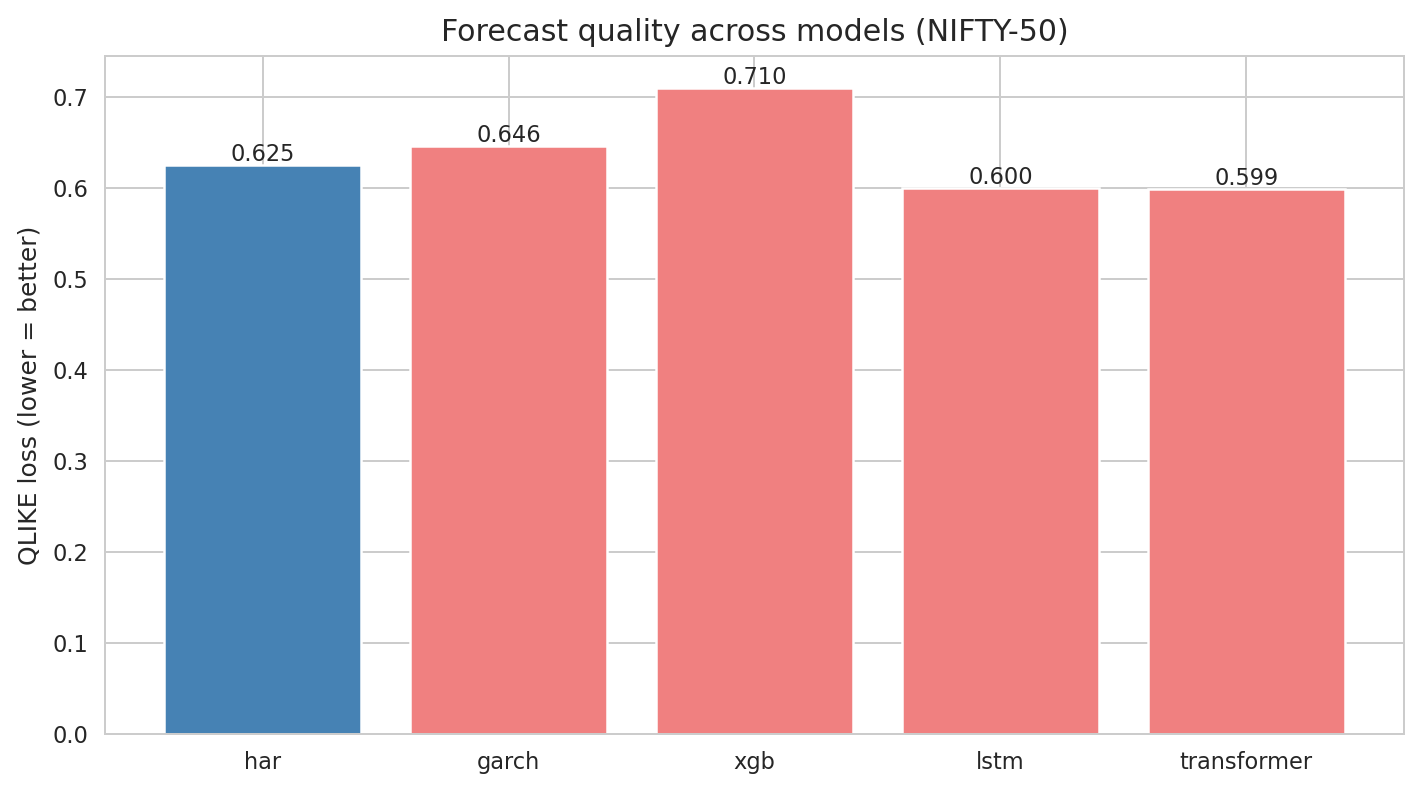
\includegraphics[width=0.85\textwidth]{../results/figures/qlike_comparison.png}
\caption{QLIKE loss across models at $h=1$. Lower is better.
Numerical differences are visible but not statistically significant
under QLIKE-based DM tests (Table~\ref{tab:dm-multihorizon}).}
\label{fig:qlike}
\end{figure}

\begin{figure}[H]
\centering
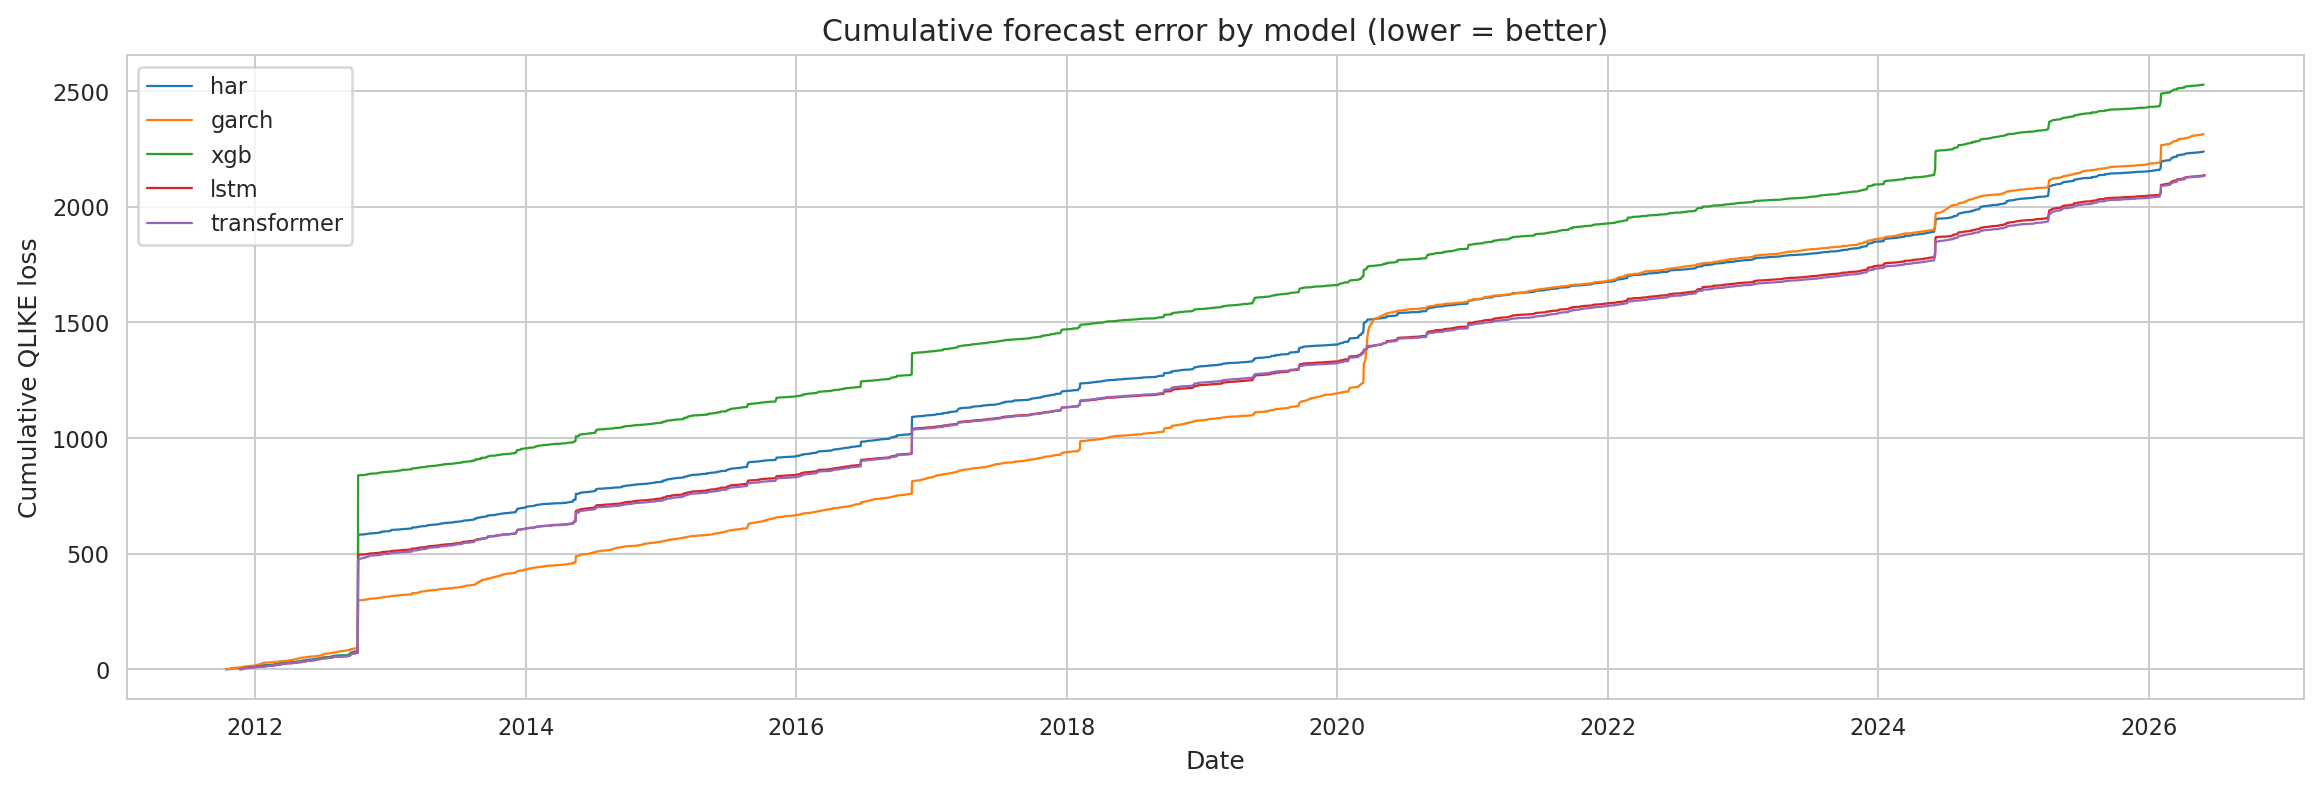
\includegraphics[width=\textwidth]{../results/figures/cumulative_loss.png}
\caption{Cumulative QLIKE loss over the out-of-sample window
($h=1$). GARCH accumulates the most loss at this horizon; HAR,
XGBoost, LSTM, and Transformer track more closely throughout.}
\label{fig:cumulative}
\end{figure}

\subsection{Robustness to LSTM hyperparameters}
\label{sec:robustness}

To assess whether the LSTM's numerical edge over HAR at $h=1$
is sensitive to specific hyperparameter choices, we run the LSTM
with varying sequence lengths and refit cadences while holding all
other settings fixed. Table~\ref{tab:robust} reports QLIKE for each
variant.

\begin{table}[H]
\centering
\caption{LSTM sensitivity at $h=1$. ``Main'' marks the configuration
used in Tables~\ref{tab:qlike-multihorizon} and~\ref{tab:dm-multihorizon}.}
\label{tab:robust}
\begin{tabular}{lrr}
\toprule
Variable & Value & QLIKE \\
\midrule
\multirow{4}{*}{Sequence length}
        & 5             & 0.595 \\
        & 10            & 0.598 \\
        & 22 (main)     & 0.609 \\
        & 44            & 0.603 \\
\midrule
\multirow{3}{*}{Refit frequency (days)}
        & 125           & 0.579 \\
        & 250 (main)    & 0.609 \\
        & 500           & 0.594 \\
\midrule
HAR-RV baseline & --- & 0.625 \\
\bottomrule
\end{tabular}
\end{table}

Across all seven configurations the LSTM QLIKE remains in the
range $[0.579, 0.609]$, below the HAR-RV baseline of 0.625. The
numerical LSTM advantage at $h=1$ is robust to hyperparameter
choice; whether this advantage rises to statistical significance
under QLIKE-DM testing for any specific configuration is left for
future work with longer time series or pooled cross-sectional data.
We note that variation across runs ($\approx 0.01\text{--}0.03$ in
QLIKE) reflects non-deterministic neural-network training and is of
comparable magnitude to the gap between HAR and the best LSTM
variant -- itself a reason for caution in over-interpreting
single-run results.

\section{Discussion}
\label{sec:discussion}

\paragraph{Why does QLIKE-based DM testing reach a different
conclusion than MSE-on-log-variance DM testing?}
The two losses weight forecast errors differently. MSE on
log-variance is symmetric in over- and under-prediction in log
space, while QLIKE penalizes underprediction much more heavily.
Models that under-predict during volatility spikes (typical for
linear and tree-based methods on heavy-tailed data) will accumulate
QLIKE loss disproportionately, while contributing modestly to
MSE-log-variance. The variance of the loss differential
$d_t = L^{\mathrm{model}}_t - L^{\mathrm{HAR}}_t$ also differs
between the two losses, with QLIKE producing wider confidence
intervals on the average loss differential on this sample.
\citet{patton2009volatility} discusses precisely this issue and
recommends that DM tests be carried out using the same loss
function as the one used for the primary forecast evaluation.

\paragraph{Reconciling with Christensen et al. (2023).}
Our numerical QLIKE results are consistent in direction with
\citet{christensen2023machine}: LSTM and Transformer have the
lowest QLIKE at $h=1$, and the GARCH advantage at $h=22$
mirrors the longer-horizon gains they report. However, our
QLIKE-based DM tests do not detect these advantages as significant,
whereas their cross-sectional panel of 30 DJIA constituents has
substantially more statistical power than our single-index design.
Two structural reasons may also play a role: first, NIFTY-50 is
a single index with a different microstructure than individual US
large-caps; second, we use the QLIKE-on-QLIKE consistency for DM
testing, which is more conservative than DM tests run on squared
log forecast errors, and the loss function used in their
significance testing may differ. We do not claim our null result
overturns Christensen et al.; we report it as a sample-power-aware
single-index replication on a market that has not previously
received systematic ML benchmarking.

\paragraph{Why is XGBoost significantly worse than HAR at $h=5$?}
At $h=5$, XGBoost is the one model with a statistically significant
DM result, and it is in the direction of being worse. A natural
explanation is that XGBoost trained on engineered HAR-style features
has all of HAR's information but also has the capacity to overfit
non-stationary feature interactions. With a target shifted further
into the future, the noise-to-signal ratio in lagged features rises,
and the additional model capacity becomes a liability rather than
an asset.

\paragraph{Limitations.}
The realized-variance proxy is itself noisy when computed from daily
OHLC data; intraday data would reduce the QLIKE floor across all
models. We use a single index (NIFTY-50) and a single set of
hyperparameters per model class; multi-asset replication would
sharpen power for any latent ML advantage. We have not conducted
ablation on model capacity (LSTM hidden size, Transformer layer
count), only on sequence length and refit cadence.

\section{Conclusion}
\label{sec:conclusion}

We have benchmarked five volatility forecasting models---GARCH,
HAR-RV, XGBoost, LSTM, and Transformer---on NIFTY-50 daily data
over 18 years at three forecast horizons (1, 5, and 22 days)
with strict walk-forward cross-validation. Using QLIKE-based
Diebold-Mariano tests for both forecast quality and significance,
we find that no model statistically beats HAR-RV at any horizon.
Numerical QLIKE gaps exist in directions consistent with theoretical
intuition (LSTM at $h=1$; GARCH at $h=22$) but lie within the
sample-noise band of DM testing.

This confirms, on Indian markets, the well-documented difficulty
of beating HAR-RV. The result also highlights a methodological
point: significance tests should be run on the same loss function
used for primary evaluation, and conclusions can change when this
discipline is enforced.

\paragraph{Future work.} Natural extensions are: (i) multi-asset
replication on individual NIFTY-50 constituents to pool power;
(ii) inclusion of macro covariates (India VIX, FII/DII flows, oil
and INR/USD); (iii) intraday data and direct realized-variance
computation; (iv) ensemble models combining HAR-RV with a
sequence-model residual correction; and (v) interpretability
analysis of which input features the LSTM and Transformer weight
most.

\paragraph{Code and data.} All code, configurations, training
scripts, and analysis notebooks are available at
\url{https://github.com/manavmishra-cloud/nifty-vol-forecast}.
NIFTY-50 OHLCV data are obtained from Yahoo Finance.

\bibliographystyle{plainnat}
\bibliography{references}

\end{document}
